\begin{figure}[b]
    	\centering
    	\begin{minipage}{0.45\textwidth}
    		\centering
    		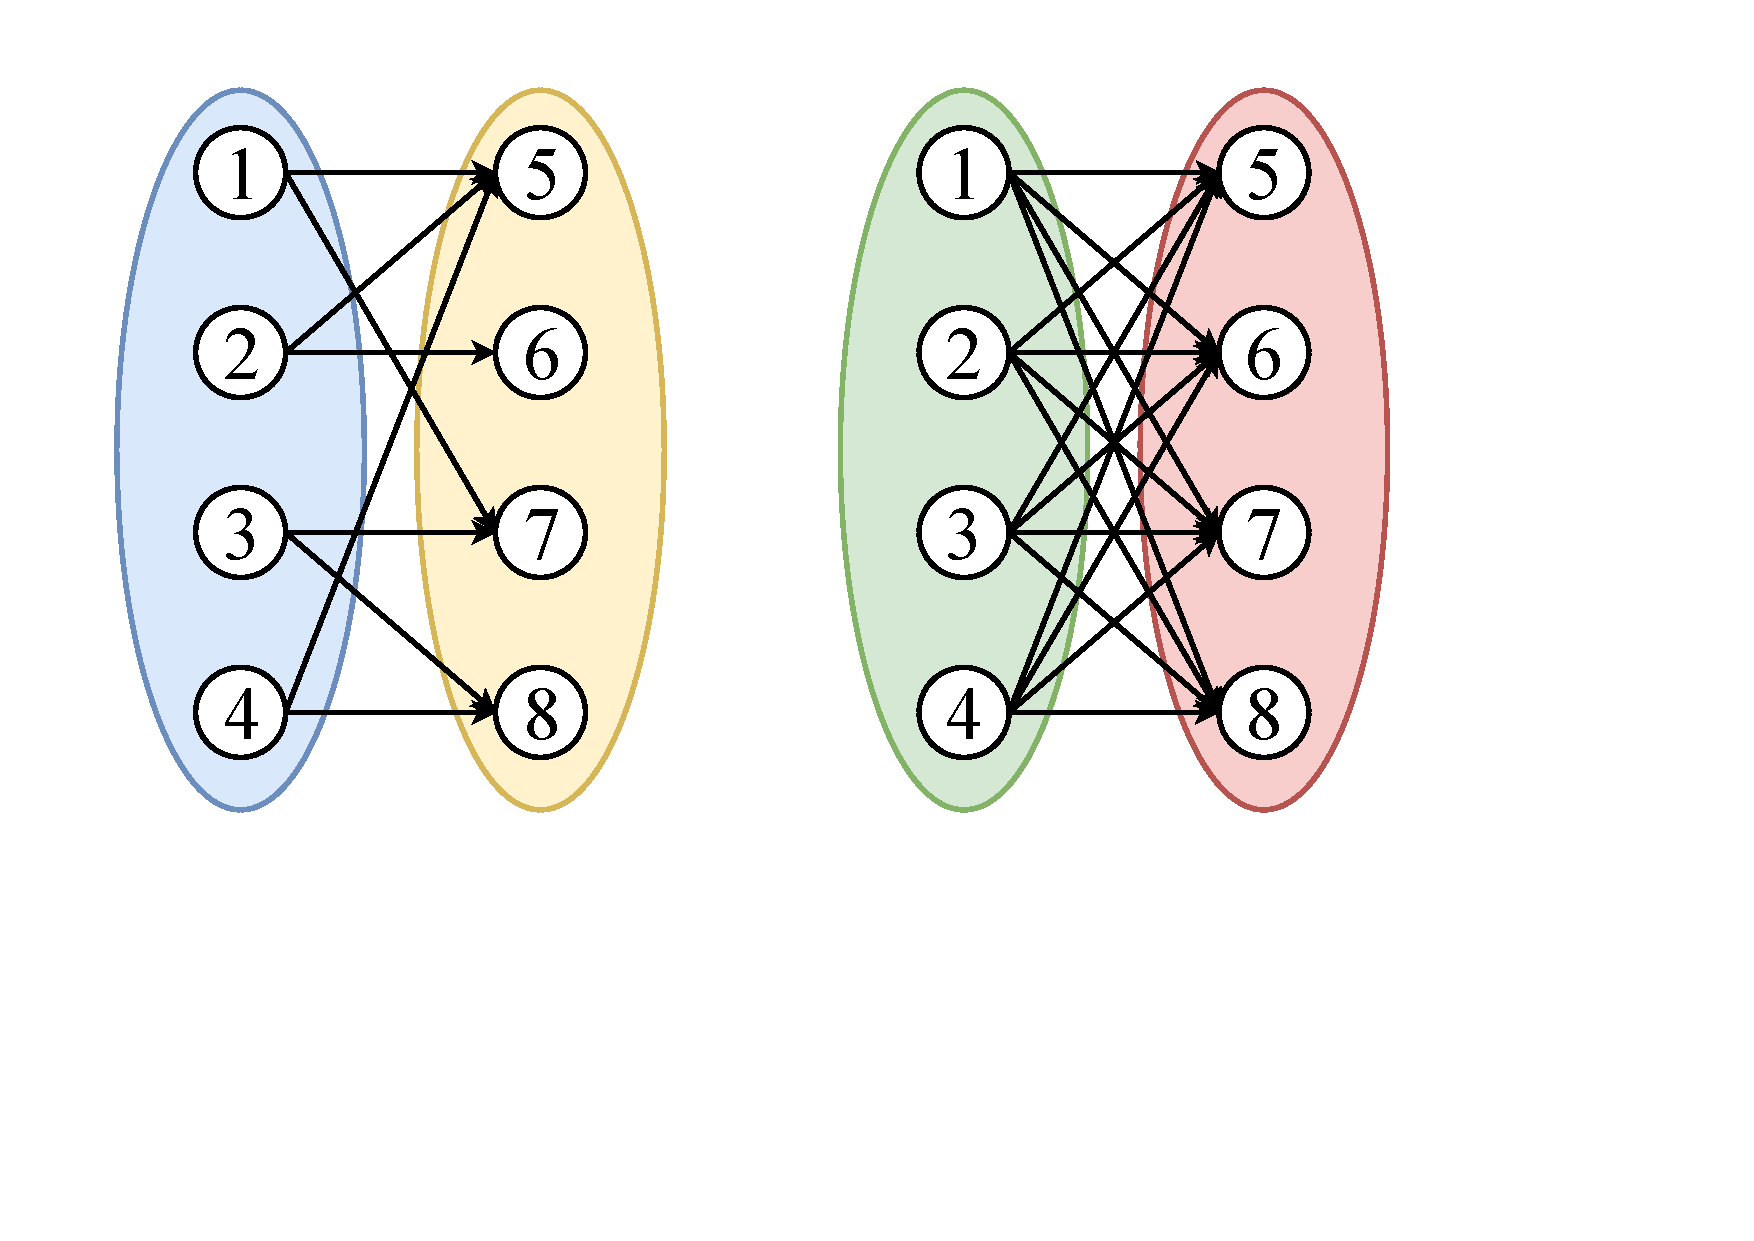
\includegraphics[scale=.3, clip,  trim=50 200 520 30]{img/graphs-bipartito.pdf}
    		
    		(a)
    	\end{minipage}
    	\begin{minipage}{0.45\textwidth}
    		\centering
    		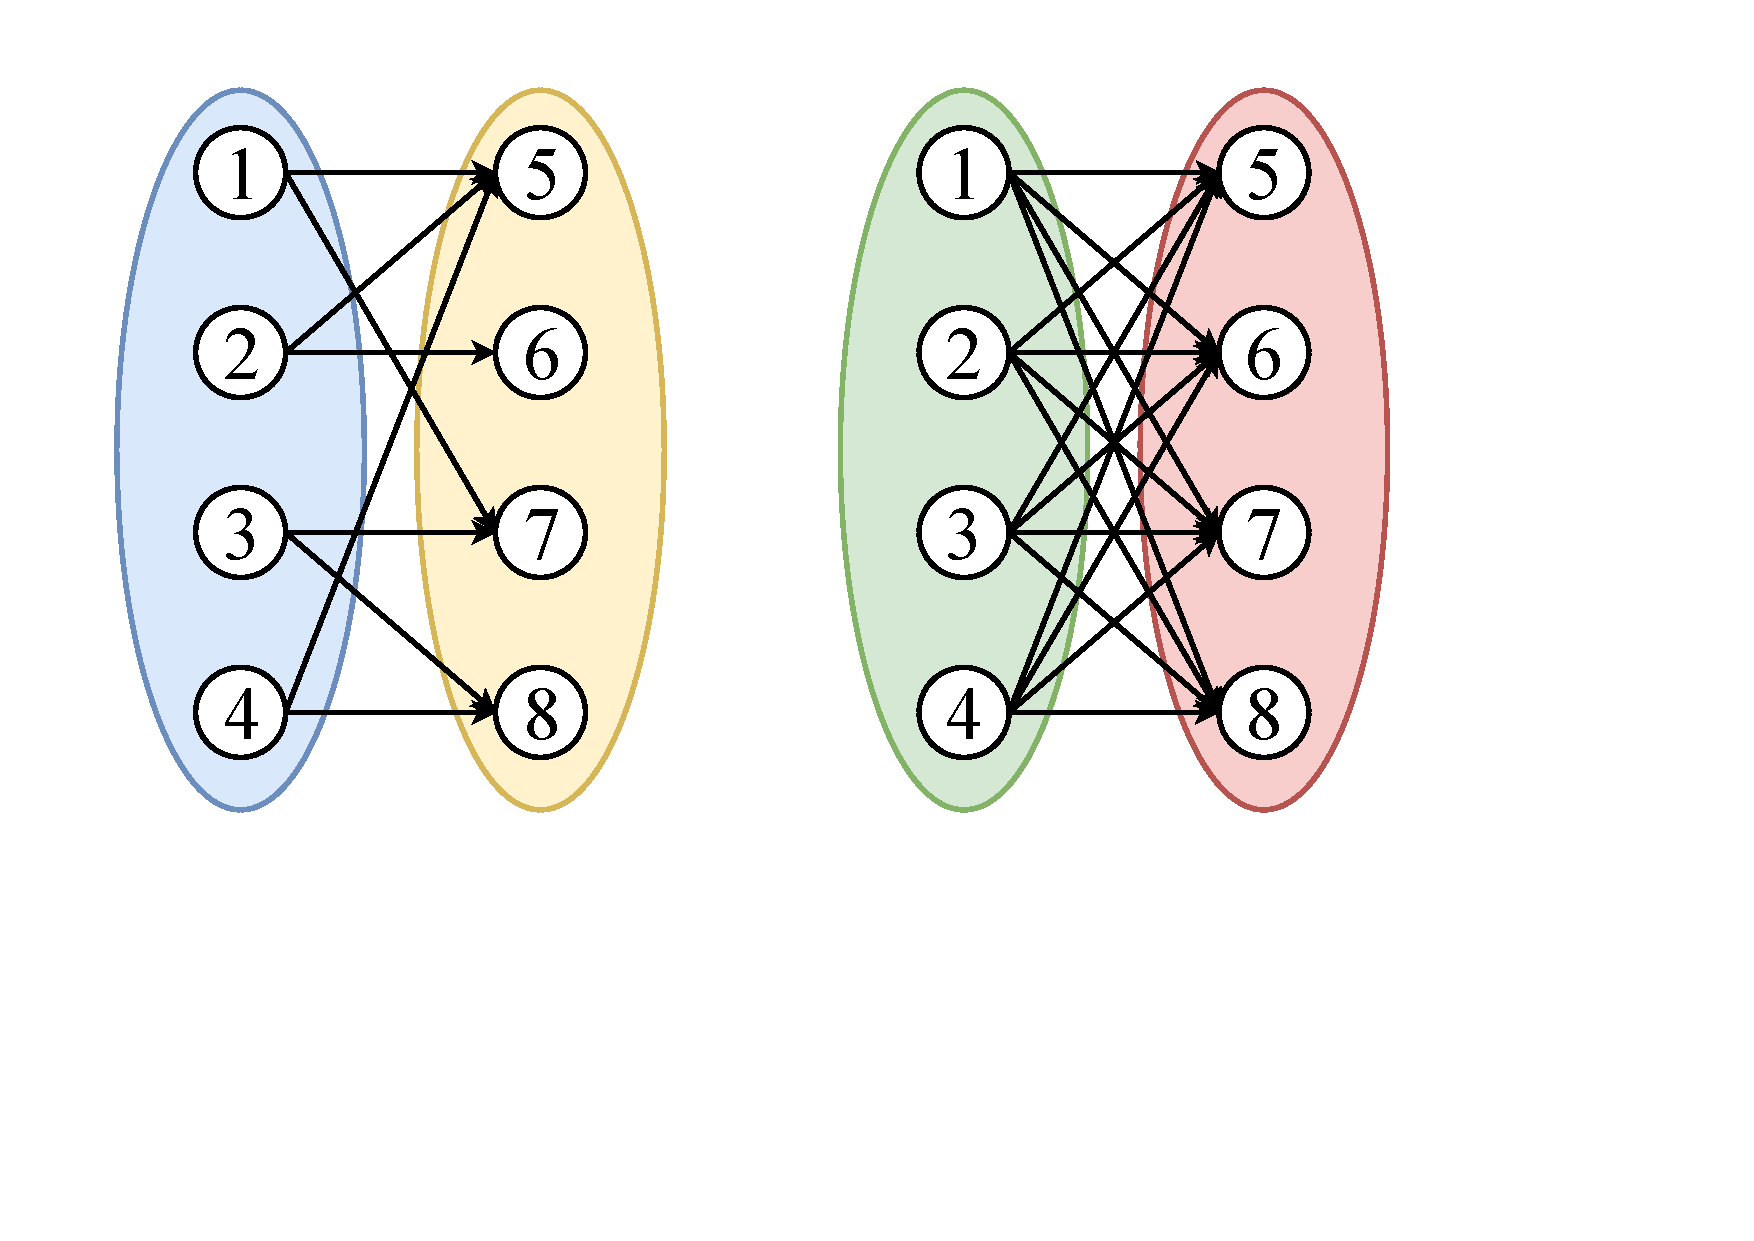
\includegraphics[scale=.3, clip, trim=400 200 170 30]{img/graphs-bipartito.pdf}
    		
    		(b)
    	\end{minipage}

    \caption{Ejemplo de grafos bipartitos. (a) Grafo bipartito. (b) Grafo bipartito completo o biclique.}
    \label{fig:bipartito}
\end{figure}
